%!TEX root = ../thesis.tex
%*******************************************************************************
%*********************************** First Chapter *****************************
%*******************************************************************************

\chapter{Introduction}  %Title of the First Chapter

\ifpdf
    \graphicspath{{Chapter1/Figs/Raster/}{Chapter1/Figs/PDF/}{Chapter1/Figs/}}
\else
    \graphicspath{{Chapter1/Figs/Vector/}{Chapter1/Figs/}}
\fi

In the automotive industry, the trend being to develop smart sensors and actuators, the on-board electronic is ever more an artful work to combine analog electronic and digital one. While many monitoring and control systems play a crucial role as well for the safety as for the comfort of passengers, small components, like ADCs, are mandatory as a building block or as an essential functionality integrated into smart actuators.

The on-board electronics is challenged by the high temperature near engine, disc brake systems and abrupt accelerations worsen the difficulty of smart actuator design. Information on automotive environments and electrical component test standards can be found at the Automotive Electronics Council web site. \figurename~\ref{fig:automotive-cond} shows the typical temperature environment for embedded electronics. The operating temperature of the electronics is a function of location, power dissipation by the electronics, and the thermal design. Noting that typical junction temperature for integrated circuits are 10\(\degree \)C to 25\(\degree \)C higher than ambient temperature, the on-engine temperature specification is often -40\(\degree \)C to 175\(\degree \)C.

\begin{figure}[htp]
    \centering
    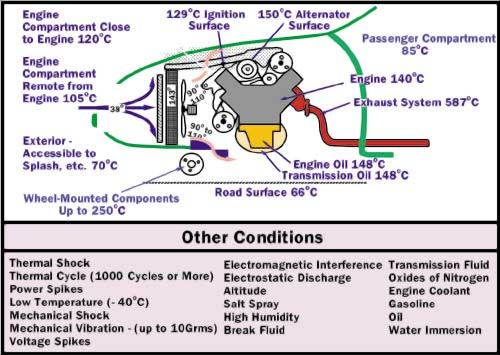
\includegraphics[width=.8\textwidth]{Chapter1/Figs/automotive_cond.png}
    \caption{Stringent automotive conditions presented by the aeconcil and backed up by~\cite{1393072,ISO16750}}
    \label{fig:automotive-cond}
\end{figure}

Despite the temperature and the other factor of stress, we are witnesses of the electrification and interconnection of our vehicles. Looking towards the vehicle-to-vehicle and the vehicle-to-infrastructure communications, information from sensors is transmit at a high pace to sustain real-time communications.

Therefore the sensor market is arguably the most important one. Among all sensors, the trends is driven by the autonomous car, and both Lidar and ToF camera are ever more developed. The Smartness of our vehicle is given by strong processing unit which could not stand the harsh environment in which most of sensors should sustain.

To transfer the information of sensors to those processing units, it is mandatory to place the Analog-to-Digital converters the closer from the sensors with a sampling rate sufficiently high for the future application of autonomous car.

%********************************** %First Section  **************************************
\section{Motivation}   % section 1.1
To that extent, a low-cost, fast and accurate analog to digital converter operating in those harsh conditions is a good ally for equipment manufacturers. To decrease the cost, the area is of primary concern. Considering re-use of the ADC as an IP-bloc, the area has been limited to less than half a square millimeter.
In the automotive environment, ADCs are the usual interface with environmental sensors and motor control sensors. 

\begin{table}[htp]
    \centering
    \caption{Specification of target ADC}
    \label{tbl:adc-spec}
    \rowcolors{2}{gray!15}{white}
    \begin{tabular}{ll}
        \toprule
                                     & Criterion                                                                                                                                                   \\ \midrule
    Operating Temperature            & -40 $\degree$ C -- +175 $\degree$ C                                                                                               \\
    Supply Voltage                   & 1.8 V $\pm$ 10 \%                                                                                                                              \\
    Differential Input Voltage Range & $\pm$ 1V                                                                                                                                       \\
    Area                             & \textless 0.5 \(mm^2\)                                                                                                                                      \\
    Conversion Speed                 & 20 MSamples/s                                                                                                                                               \\
    Maximum Clock Frequency          & 100 MHz
    Clock Duty-Cycle                 & 40 -- 60 \%                                                                                                                                                 \\
    Latency                          & 500 ns                                                                                                                                                      \\
    Resolution                       & $\geq$ 12-bits                                                                                                                                     \\
    \rowcolor{white}                 & $F_s$ \textless 5 MHz, min 74 dB\\
    \rowcolor{white}                 & 5 MHz \textless $F_s$  \textless 10 MHz, min 68 dB\\
    \rowcolor{white}\multirow{-3}{*}{SNDR } & $F_s$  \textgreater 10 MHz 62 dB \\
    SFDR (Full-Scale)                & min 68 dB                                                                                                                                                   \\
    DNL                              & \textless LSB/2                                                                                                                                             \\
    INL                              & \textless LSB/2 best-fit method                                                                                                                             \\
    Offset Error                     & \textless 4 LSB                                                                                                                                             \\
    Gain Error                       & \textless 4 LSB                                                                                                                                             \\
    Adjacent ADC mismatch Error      & \textless 4 LSB                                                                                                                                             \\
    Energy, $E_s = P/F_s$            & 0.75 nJ/sample      \\ \bottomrule                                                                                                                                       
    \end{tabular}
\end{table}

\nomenclature[z]{PVT}{Process-Voltage-Temperature}
The frequency spectrum of such application being limited, the ADC does not need to tackle for Gigahertz sampling. The accuracy and the linearity is of much importance. Nevertheless, vehicle communicates the sensors information. To receive them, the bandwidth of the signal is few megahertz.
To fulfill the need, the minimum requirements for a final product are listed in Table~\ref{tbl:adc-spec}. The order of importance is the area, the resolution, the power consumption, and the conversion speed. It is important to highlight the temperature range and the ratio between the conversion speed and the maximum clock frequency equal to 5. This ratio also called Oversampling Ratio (OSR) is the number of clock cycle allowed to perform a conversion.

To responds to the future need of the automotive environment, we aim a design of an ADC over a wide temperature range from -40\(\degree \)C to 175\(\degree \)C with the following characteristics:

\begin{itemize}
\item Maximum oversampling ratio of 5
\item SNDR greater than 68 dB
\item a consumption less than 0.75 nJ/sample
\item and target a silicon area less than 0.5 \(mm^2 \) for cost reason
\end{itemize}
 
With a preference sets on the minimization of the silicon area, before the minimization of the power consumption, the resolution and the speed.

\section{Thesis Contribution}

This work focuses on the design of high-precision, high-speed and energy efficient ADC under the harsh environment the automotive one represents. A particular emphasis is on doing such design in a SOI CMOS processes under stringent Process-Voltage-Temperature (PVT) variations. Our main contribution relies on the development of an new hybrid topology proposal using 3 stages to cope with such constraints based on a top-down approach: A first counting stage inherently linear, an algorithmic stage allowing to increase rapidly the precision, and a SAR stage, ideal in terms of area and consumption, for a low number of bits.

In this regard, we review operation of conventional ADC topologies in the Chapter~\ref{sec:soa}. Their advantages and source of errors are discussed to present why some architectures are predominant in high temperature conditions. Namely, few of them such as \(\Delta \Sigma\), SAR, and pipelined are able to cope with analog imperfections coming from the temperature. The proposed architecture is then presented to benefit from the strength of each one.

The section~\ref{sec:temperature-analogue} then discusses the challenge of analog design over a large temperature range from -40\(\degree\)C to +175\(\degree\)C. Phenomena tightly linked to the temperature are analysed to highlight the design trade-offs when considering temperature effects. Based on a \(g_m/I_D\) methodology, the insight gained from this analysis is then reused during the conception phase.

Having the severe degradation the analog undergoes, we discuss enhancement ported to our topology proposal to glean the maximum of performances within the smallest footprint in a 180 nm technology. Alongside the optimization, Chapter~\ref{sec:adc-implementation} considers the reliability and introduces the case of pseudo-asynchronous design to relax timing restrictions in the digital part over temperature. We have defined a methodology for the design and characterization of such converter by using a testbench comparing a high-level model of the converter, defined in VerilogAMS, and a schematic description of the converter, able to use macromodels of the components or their transistor-level description. A MATLAB post-processing is able to extract the main characteristics such as the precision, the INL, DNL ...

The design of mandatory analog blocks, which are respectively comparators and operation amplifier, is examined to ensure the expected behaviour for a rigorous 6\(\sigma\) process variation. In order to achieve this, a new time delay model have been developed for the Double Tail latch. This model has been presented during the ECCTD conference held in 2017. Meanwhile, the layout concerns to get the most of the op-amp is also discussed in the Chapter~\ref{sec:analog-building-bloc}.

Despite the fact the ADC testchip is in a finalization stage, experimentation is key in the validation process of IP components. Details in the realization of test in temperature which are worth to be discussed are presented in Chapter~\ref{sec:tests-meas}. In this regard, the delay of high speed clocked comparator have been measured. The original delay measurement circuits, also presented during the ECCTD in 2017, is presented and compared to conventional circuits to measure the time elapsed. After the enhancement of our topology proposal, only the testability of the last stage has seen its complexity increased. Therefore, this chapter dives into the its specificities of measurement, while static performance metrics demonstrate the effectiveness of pseudo-asynchronous design at high temperature. Chapter~\ref{sec:perspectives} concludes our research findings and suggests potential future work.
